\documentclass{article}
\usepackage{natbib}
\usepackage[labelfont=bf]{caption}
\usepackage{subcaption}
\usepackage{graphicx}
\usepackage{float}
\bibliographystyle{apalike}
\usepackage{lineno}
\linenumbers

\usepackage{geometry}
\geometry{letterpaper}
\geometry{margin=1in}

\usepackage{setspace}
\doublespacing
\captionsetup[figure]{font={stretch=2}}

\usepackage{authblk}
\usepackage{xcolor}

\newcommand{\matr}[1]{\mathbf{#1}}

%\title{Improving Accuracy of Simulated Flows in Steeply Dipping Layers Using Full-Connectivity Grids with the XT3D Multi-Point Flux Approximation in MODFLOW 6}

% suggested title revision
\title{Efficient and Accurate Modeling of Flow through Sedimentary Structures with MODFLOW 6}

\author{
	Alden M. Provost, U.S. Geological Survey, Integrated Modeling and Prediction Division, U.S. Geological Survey, 12201 Sunrise Valley Dr, Reston, VA, USA  \\
	\and 
	Kerry Bardot, School of Earth Sciences, University of Western Australia, Perth, Australia \\
	\and 
	Christian D. Langevin, U.S. Geological Survey, Integrated Modeling and Prediction Division, 2280 Woodale Drive, Mounds View, MN, USA \\
	\and 
	James L. McCallum, School of Earth Sciences, University of Western Australia, Perth, Australia \\
	}


\date{\today}

\begin{document}

\maketitle

\textbf{Conflict of interest:} None.

\textbf{Key words:} groundwater flow simulation, sedimentary structures, dipping layers, full-connectivity grid {\color{red} AMP: maybe ``cell connectivity''' or ``grid connectivity'' would make a better search term?}, multi-point flux approximation

\textbf{Article impact statement: Groundwater flow through dipping sedimentary structures can be accurately simulated using the XT3D multi-point flow formulation in MODFLOW 6.}

\begin{abstract}
Groundwater flow through dipping hydrogeologic layers is often modeled with MODFLOW by specifying top and bottom elevations of model layers to coincide with top and bottom elevations of hydrogeologic layers.  With this approach, adjacent cells within a model layer are vertically offset from one another.  While the standard formulation in MODFLOW does not rigorously account for these offsets in the underlying flow calculations, results are generally expected to be accurate provided dip angles do not exceed $10^{\circ}$.  To improve the accuracy of flow simulations on unstructured grids, and to allow accurate simulation of arbitrarily oriented two- or three-dimensional anisotropy, the optional XT3D multi-point flow formulation was introduced in MODFLOW 6.  The XT3D flow formulation is designed to account for geometric irregularities in the grid, including vertical offsets between laterally adjacent cells, and to provide accurate results for both isotropic and anisotropic groundwater flow.  \cite{bardot2022} showed, however, that neither the standard formulation nor the XT3D formulation produced the correct flow direction and magnitude in simple tests involving flow through a steeply dipping, permeable hydrogeologic layer.  In this paper, we explain that the inability of XT3D to give accurate results in the steeply dipping test problem of \cite{bardot2022} was caused by the limited cell connectivity that is inherent in the most commonly used discretization packages in MODFLOW 6. The DIS and DISV discretization packages are based on layered connectivity in which cells have lateral connections only with cells in the same grid layer.  We demonstrate that layered lateral connectivity is insufficient to allow accurate simulation of flow through a steeply dipping hydrogeologic layer on a vertically offset grid.  When lateral connections between cells in adjacent grid layers are included using the fully unstructured (DISU) grid type, XT3D is able to calculate the flow magnitude and direction accurately for both isotropic flow and for anisotropy oriented along the permeable hydrogeologic layer.  To realize this improved accuracy, the permeable hydrogeologic layer must be discretized vertically using at least two model layers. {\color{red} (AMP: Given the idealized nature of the test problem, how general can we be with our conclusions? I pulled it back here relative to what you had originally, CDL, but left a slightly stronger statement in the Conclusions, at least for now.})  Our findings suggest that, given appropriate discretization and cell connectivity, the combination of vertically offset grids with the XT3D flow formulation in MODFLOW 6 can provide a computationally efficient and accurate method for simulating isotropic and anisotropic flow through steeply dipping sedimentary structures, a capability that was previously reserved to finite-element-based simulators. {\color{red} (AMP: Any Pal and Edwards-type MPFA stuff that's relevant to that final phrase? See also Conclusions)}
\end{abstract}

\section{Introduction}

In the MODFLOW family of hydrologic simulation codes, a groundwater model domain is discretized into a grid of hydraulically connected model cells. Versions of MODFLOW up to and including MODFLOW-2005 \citep{modflow2005} offered only structured grids composed of rows, columns, and layers of cells. Cells were conceptualized as having horizontal top and bottom surfaces and vertical lateral faces, which allowed each cell to be ``simulated as if it were rectangular so that flow may be approximated by the standard finite-difference equation'' \citep{modflow84}. In MODFLOW-USG \citep{modflowusg} and MODFLOW 6 \citep{modflow6gwf}, which offer unstructured grids and use the control-volume finite-difference method to formulate the discrete balance equations, cells continue to have horizontal tops and bottoms and vertical lateral faces.  Defining cells with horizontal tops and bottoms and vertical lateral faces simplifies the definition and calculation of water-table elevations, cell saturations, hydraulic conductances between cells, and transitions between confined and unconfined conditions.

A traditional approach to representing an aquifer system with dipping hydrogeologic layers in MODFLOW is to map the hydrologic properties onto a rectilinear grid \citep{modflow84}.  \cite{hoaglund2003} refer to this as the ``grid overlay'' method.  In the grid overlay method, the boundaries of dipping hydrogeologic layers are represented approximately, in what \cite{bardot2022} call a ``staircase'' fashion.  Another approach available in all versions of MODFLOW is to allow the top and bottom elevations of cells in the same layer of the grid to vary spatially. Following \cite{bardot2022}, we call this type of grid ``vertically offset.'' In this work, we show how to improve the accuracy of flow simulations that use vertically offset grids. The vertical offsets in top and bottom elevations between adjacent cells within a grid layer allows each grid layer to ``deform'' with the hydrostratigraphy. This ``minimize[s] the number of model [grid] layers required to simulate an aquifer system'' \citep{modflow84} relative to the grid overlay method.

All versions of MODFLOW prior to MODFLOW 6 used a two-point, ``conductance-based'' flow formulation in which the flow between two adjacent cells is proportional to the difference between the heads calculated in those two cells. The conductance-based flow formulation is most accurate when the grid satisfies the ``control-volume finite-difference (CVFD) requirement'' that the straight-line connection between two cell centers must intersect the midpoint of the cell-cell interface at a right angle \citep{narasimhan1976integrated}. However, vertically offset grids violate the CVFD requirement because lateral cell faces are vertical but cell connections are not strictly horizontal. For this reason, the MODFLOW 6 documentation \citep{modflow6gwf} warns that ``[s]teeply dipping layers generally should not be represented'' using vertical offsets. \cite{anderson2015applied} recommend a $10^{\circ}$ dip as a practical upper limit for using vertical offsets.

To improve the accuracy of flow simulations on unstructured grids, and to allow accurate simulation of arbitrarily oriented two- or three-dimensional anisotropy, the optional XT3D flow formulation \citep{modflow6xt3d} was introduced in MODFLOW 6. By performing flow calculations using Darcy's Law in its tensorial form based on a multi-point approximation of the head gradient vector, XT3D accounts for both arbitrarily oriented anisotropy and geometric irregularity of the grid. In theory, XT3D should be able to compensate for the geometric irregularity introduced by vertical offsets between adjacent cells in the same grid layer.

\cite{bardot2022} evaluated the effects of grid design and XT3D on the ability of MODFLOW 6 to accurately simulate flow through sedimentary structures by modeling an idealized, two-dimensional permeable feature (``channel'') in plan view and a dipping hydrogeologic layer (which \cite{bardot2022} also generically called a ``channel'') in cross-section. {\color{red} (CDL: use ``permeable feature'' instead of channel?) (AMP: Think it's ok to use channel here in reference to Kerry and Jim's plan-view model, but not after this paragraph; made changes to that effect throughout.)} In each case, the channel or hydrogeologic layer was embedded in a nearly impermeable surrounding medium, or ``domain.'' In their plan-view benchmark, the channel lay within the horizontal plane and was angled counterclockwise relative to the southern boundary of the model (by $30^{\circ}$ in most cases). Constant-head boundary conditions at the ends of the channel were set to induce uniform flow along the channel in the corresponding analytical solution. The channel and surrounding domain were discretized using either a rectilinear grid, which satisfies the CVFD requirement, or a ``flexible triangular'' grid that is unstructured with triangular cells that conform to the channel boundary but does not satisfy the CVFD requirement. They found that the standard, conductance-based flow formulation gave accurate results on the rectilinear grid using isotropic hydraulic conductivity tensors (although accuracy decreased substantially in the presence of anisotropy) but was subject to significant error on the unstructured grid. By contrast, the XT3D flow formulation gave accurate results on both grids for both isotropic and anisotropic hydraulic conductivity tensors, as expected. However, in the cross-sectional (``transect'') version of their benchmark, which used a vertically offset grid to discretize the nearly impermeable domain and a highly permeable hydrogeologic layer inclined by $30^{\circ}$ from the horizontal, similarly poor results were observed with and without XT3D. Given the ability of XT3D to compensate for violations of the CVFD requirement, it appeared likely that another aspect of the problem formulation or the inner workings of MODFLOW 6 was responsible for the unexpected results.  As noted by \cite{bardot2022}, a preliminary analysis by two authors of the present work (Provost and Langevin) suggested that the limited cell connectivity offered by the vertically offset grid was inadequate for allowing an accurate flow solution.

MODFLOW 6 supports three different types of grids: regular MODFLOW grids consisting of layers, rows, and columns (DIS);  grids discretized by vertices (DISV); and fully unstructured (DISU) grids, which are patterned after the DISU grid type in MODFLOW-USG  \citep{modflowusg}.  The DIS and DISV grids in MODFLOW 6 are ``layered'', which means that the same two-dimensional grid structure (in plan view) applies to all grid layers.  The ``layered'' concept of DIS and DISV grids is used within MODFLOW to determine how cells are hydraulically connected.  Cells in DIS and DISV grids are automatically assigned vertical connections to overlying and underlying cells and horizontal connections to adjacent cells in the same grid layer.  DISU grids are more flexible than DIS and DISV grids in that the user has complete freedom to specify the cell connectivity and the geometric properties for each connection.  DISU grids support two types of horizontal connections: a ``layered'' horizontal connection and a ``vertically staggered'' horizontal connection \citep{modflow6gwf}.  With a layered horizontal connection, the hydraulic conductance is calculated using the full saturated thicknesses of the two connected model cells.  By contrast, for a staggered horizontal connection, the hydraulic conductance is calculated using only the area of overlap between the two cell faces. Vertically staggered horizontal connections were introduced in MODFLOW-USG \citep{modflowusg} and included in MODFLOW 6 \citep{modflow6gwf} primarily as a means to vertically subdiscretize parts of a model domain.  Vertically staggered connections offer the possibility of implementing ``full'' connectivity in the sense that every cell is hydraulically connected to every other cell with which its faces overlap.

The grid used by \cite{bardot2022} for the steeply dipping benchmark example used layered horizontal connections.  To our knowledge, the implications of limited horizontal connectivity in layered grids for the accuracy of simulated flows in models with steeply dipping hydrogeologic layers, and the potential for using full cell connectivity via vertically staggered connections to overcome this limitation, have not been previously appreciated or investigated.

% text removed
% For a grid that includes vertically staggered connections, which in this work we call a ``vertically staggered grid,'' some cells have nominally ``horizontal'' connections with more than one cell in some direction. Vertically staggered DISU grids allow more flexibility in assigning cell connectivity than do the more commonly used DIS and DISV grid types \citep{modflow6gwf} in MODFLOW 6. 

In the remainder of this paper we first present a theoretical justification for the hypothesis that inadequate cell connectivity is primarily responsible for the inaccurate simulation of flows in the steeply dipping hydrogeologic layer benchmark on a vertically offset grid. Based on that theory, we propose a method for improving the accuracy of the flow solution using XT3D together with vertically offset grid with full connectivity, and we evaluate the effectiveness of that approach in a set of benchmark problems similar to those of \cite{bardot2022}. Finally, we discuss the potential implications of our findings for practical groundwater models that include high permeability contrasts and steeply dipping hydrogeologic layers.

{\color{red} (AMP: Work in the reference Jim found and our recent MF6 overview paper somewhere?)}

\section{Theoretical Background}

\begin{figure}
	\begin{center}
	\includegraphics[scale=0.6]{../figures/schem_conn_area_flux.png}
	\caption{Schematics showing (a) cell connectivity and (b) cell-cell interface fluxes in a two-grid-layer model of a dipping hydrogeologic layer. Hatching denotes impermeable boundaries along the top and bottom of the hydrogeologic layer. In (a), black circles represent cell centers. Blue lines represent hydraulic connections between cells in a layered-connectivity grid. Red lines represent additional connections that must be made to achieve full connectivity. In (b), gray arrows represent the uniform groundwater flux the model is attempting to simulate. Blue arrows represent components of the uniform groundwater flux normal to the horizontal and vertical cell-cell interfaces in the layered-connectivity grid. Red arrows represent components of the uniform groundwater flux normal to the additional vertical cell-cell interfaces introduced to represent the full connectivity.}
	\label{fig:schem-conn-area-flux}
	\end{center}
\end{figure}

Figure \ref{fig:schem-conn-area-flux}a shows a group of four cells in a two-grid-layer, cross-sectional MODFLOW 6 model of fully saturated flow through a permeable hydrogeologic layer (aquifer) with impermeable top and bottom boundaries. The cells have horizontal tops and bottoms and can therefore follow the dip of the hydrogeologic layer only on average. If the grid is represented using a layered grid type (DIS or DISV) in MODFLOW 6, a cell is hydraulically connected to each adjacent cell in the same grid layer, regardless of whether or not the cells overlap, and with each overlying and underlying cell, as indicated by the blue lines that connect cell centers in Figure \ref{fig:schem-conn-area-flux}a. In this work we call this a vertically offset grid with ``layered connectivity.''  Note that cells that have overlapping vertical faces but are in different grid layers (e.g., cells 1A and 2B) do not have a direct hydraulic connection in a grid with layered connectivity. The addition of such connections between cells in different grid layers, as indicated by the red lines that connect cell centers in Figure \ref{fig:schem-conn-area-flux}a, results in a grid with ``full connectivity.''  In MODFLOW 6, only layered connectivity can be represented in structured (DIS) and vertex-based (DISV) grids. Fully unstructured (DISU) grids allow representation of any kind of cell connectivity, including layered or full connectivity.

The default method for representing the flow between two hydraulically connected model cells in MODFLOW 6 is the ``conductance-based flow formulation'' \citep{modflow6gwf}. In this formulation, which is based on the commonly used two-point flux approximation {\color{red} *** ref? ***}, the flow is proportional to the difference in the hydraulic heads computed at the two cell centers and a hydraulic conductance based on an effective hydraulic conductivity for the connection between the cells. On strictly rectilinear grids, such as structured MODFLOW grids with no vertical offset between cells in the same grid layer, with hydraulic conductivity that is isotropic or has anisotropy aligned with the three mutually perpendicular grid directions, the conductance-based formulation is second-order accurate \citep{dehotin2010modeling, modflow6gwf}. This is because strictly rectilinear grids satisfy the ``control-volume finite-difference (CVFD) requirement'' that the straight-line connection between two cell centers must intersect the midpoint of the cell-cell interface at a right angle \citep{narasimhan1976integrated}. However, vertically offset grids violate the CFVD requirement because nominally ``horizontal'' connections between cell centers in the same grid layer are not strictly horizontal and therefore not perpendicular to the vertical cell-cell interfaces they intersect. For example, in Figure \ref{fig:schem-conn-area-flux}a, the connection between cells 1A and 1B is not perpendicular to the cell-cell interface, which compromises the accuracy of the conductance-based formulation.

The conductance-based formulation was the only flow formulation available in versions of MODFLOW prior to MODFLOW 6. As mentioned earlier, the limitations of the conductance-based formulation on vertically offset grids were well recognized. However, the ability to use unstructured grids in MODFLOW-USG and MODFLOW 6 introduced new ways to violate the CVFD requirement, and thereby render the conductance-based formulation less accurate, even in the absence of vertical offsets. The concept of a ``ghost node'' was included in MODFLOW-USG \citep{modflowusg}, and subsequently in MODFLOW 6, as a simple and optional way to improve the accuracy for grids that violated the CVFD requirement.  However, implementation of the ghost-node correction is highly problem dependent, and it is not obvious how to specify optimal ghost-node locations and weights on complex, unstructured grids.  As a more ``automatic'' alternative to the ghost-node method for improving accuracy, and as a way to allow accurate simulation of arbitrarily oriented two- or three-dimensional anisotropy, the optional XT3D flow formulation \citep{modflow6xt3d} was introduced in MODFLOW 6.  XT3D formulates the flow between two cells by interpolating head values from the two cells and their neighboring cells to construct an estimate of the full, two- or three-dimensional head-gradient vector on each side of the cell-cell interface; applying the cell conductivity tensors to obtain an estimate of the groundwater flux  normal to the interface on each side of the interface; and reconciling the two flux estimates to ensure continuity of flow across the interface. By performing flow calculations using Darcy's Law in its tensorial form, based on a ``multi-point'' approximation of the head gradient, XT3D accounts for both arbitrarily oriented anisotropy and geometric irregularity of the grid.

The dipping-hydrogeologic-layer benchmark problem of \cite{bardot2022} used a vertically offset layered grid, which is the type of grid used most often in MODFLOW models. Test simulations using the conductance-based flow formulation for a steeply dipping hydrogeologic layer (which we will call the ``aquifer'') embedded in a domain that is six orders of magnitude less hydraulically conductive yielded significant errors in the simulated flows. The simulated groundwater flux in the middle of the aquifer was not along the $30^{\circ}$ incline of the aquifer as expected, but nearly horizontal ($0.03^{\circ}$ incline), and its magnitude was overestimated by 15\%. Significant errors in the simulated flows were expected in this case, given that the conductance-based flow formulation does not rigorously account for violations of the CVFD requirement that the cell-cell connection be perpendicular to the cell-cell interface, and that it takes the connection length to be the horizontal distance between cell centers.  Given the ability of XT3D to account rigorously for cell connections that are not perpendicular to cell-cell interfaces, and for the increase in connection length due to the slope of the connection, rerunning the simulation with XT3D activated could have been expected to improve the flow solution substantially. However, \cite{bardot2022} observed similarly poor results with XT3D: the flux was still nearly horizontal ($0.01^{\circ}$ incline), and its magnitude was overestimated by 12\%. Based on a preliminary analysis by two authors of the present work (Provost and Langevin), \cite{bardot2022} hypothesized that the unexpectedly large error in the flow solution with XT3D was related to inadequate cell connectivity.

The role of cell connectivity in enabling accurate simulation of flow along a dipping hydrogeologic layer can be understood by considering Figure \ref{fig:schem-conn-area-flux}b, in which components of the groundwater flux (specific discharge) vector representative of steady, uniform flow along the hydrogeologic layer are superimposed on each cell-cell interface. Gray vectors represent the uniform flux oriented along the hydrogeologic layer, which the model is attempting to simulate. Blue vectors represent the flux components normal to cell-cell interfaces that correspond to blue connections in Figure \ref{fig:schem-conn-area-flux}a, which are common to both the layered-connectivity and full-connectivity grids. Red vectors represent the flux components normal to cell-cell interfaces that correspond to red connections in Figure \ref{fig:schem-conn-area-flux}a, which are lacking in the layered-connectivity grid.

The blue vectors in Figure \ref{fig:schem-conn-area-flux}b show that to simulate steady, uniform flow along the dipping hydrogeologic layer, cells must exchange water not only ``horizontally'' with neighboring cells in the same grid layer, but also vertically with cells in the adjacent grid layer. Specifically, there must be flow from cells in the bottom grid layer to cells in the top grid layer, which corresponds to the vertical component of the groundwater flux. Note, however, that the blue vectors alone are incompatible with steady, uniform flow along the hydrogeologic layer because the exchange of water between the two grid layers is in one direction only: upward. Such a steady-state flow configuration would imply continuous depletion of flow within the bottom grid layer and accumulation of flow within the top grid layer as one moves along the hydrogeologic layer in the direction of flow. Thus, steady, uniform flow along the hydrogeologic layer cannot be simulated accurately without some mechanism for returning flow from the top grid layer to the bottom grid layer. The full-connectivity grid provides such a mechanism by offering additional connections between cells in adjacent grid layers. Vertical flows from the bottom grid layer to the top grid layer, represented by vertical blue vectors in Figure \ref{fig:schem-conn-area-flux}b, can be returned to the bottom grid layer by nominally ``horizontal'' flows, represented by red vectors in Figure \ref{fig:schem-conn-area-flux}b. Although this concept has been illustrated using a two-grid-layer model for simplicity, the same reasoning applies given any number of grid layers.

Once the full connectivity is established, it is the role of the flow formulation to account properly for the geometry of the grid, a task for which XT3D was specifically designed. However, XT3D alone cannot compensate for cell connectivity that does not provide adequate pathways for flow. This explains why using XT3D did not improve the simulation results substantially on the layered-connectivity grid in the benchmark tests of \cite{bardot2022}.  In the middle section of the hydrogeologic layer, away from the end boundary conditions, the flow solution approached steady, uniform flow the only way that it could given the limited connectivity: by suppressing vertical flows between grid layers, thereby rendering the overall flow approximately horizontal.

The arguments presented in this section suggest that, in addition to the use of XT3D, full connectivity can be important for obtaining an accurate flow solution in MODFLOW 6 simulations that involve steeply dipping hydrogeologic layers. The next section presents results of simulations designed to test this hypothesis.

\section{Description of Test Problem}

The test problem is patterned after the cross-sectional (transect) benchmark of \cite{bardot2022}. It attempts to simulate uniform flow in an inclined permeable hydrogeologic layer (``aquifer'') embedded in less permeable material (the ``domain'').

To simulate flow along an aquifer of uniform thickness inclined at angle $\theta$ relative to the horizontal ($30^{\circ}$ for the base case), heads are specified at the centers of cells along the perimeter of the model using a formula that corresponds to a uniform, unit head gradient:
\begin{equation}
\label{eqn:head_analyt_along}
h = - x \cos \theta - z \sin \theta.
\end{equation}

\noindent where $h$ is head in meters and $x$ and $z$ are the horizontal and vertical model coordinates, respectively, in meters. The hydraulic conductivity of the aquifer is set to 1 m/d (meter per day) so that the analytical flow solution is a groundwater flux of 1 m/d along the aquifer. In the base case, the conductivity of the domain surrounding the aquifer is set to $10^{-6}$ m/d to effectively isolate the aquifer hydraulically.

Two methods of discretization are used to simulate the test problem: (1) vertically offset grid of the MODFLOW 6 DIS (structured) type, and (2) vertically offset grid of MODFLOW 6 DISU (unstructured) type. The cell geometry in these two discretization methods is identical, but the cell connectivity is different. The DIS grid uses layered connectivity, and the DISU grid includes the additional connections between cells in adjacent grid layers needed to realize full connectivity. The DISU grid is constructed by starting with a DIS grid, converting it to an equivalent DISU grid, and then implementing full connectivity. The base case uses grids consisting of 11 columns and 9 layers of cells, with 3 layers within the aquifer, 3 layers in the domain above the aquifer, and 3 layers in the domain below the aquifer. {\color{red} (AMP: Need dimensions of aquifer and domain.)}

The above description represents the base-case test problem. However, the results also include simulations designed to investigate the effects of varying the gridding resolution, the dip angle of the aquifer, the conductivity contrast between the aquifer and the domain, and the anisotropy of the conductivity tensor.

Jupyter notebooks created for the test problem are available in the Supporting Information that accompanies this paper. The notebooks leverage the capabilities of FloPy \citep{bakker2016scripting, hughes2023flopy} to assist in setting up input for and processing results from the MODFLOW 6 simulations. A Python script for converting structured, DIS grids to unstructured, DISU grids with full connectivity is included.

\section{Results and Discussion}

{\color{red} (AMP: Did some editing of this section for flow and consistent style, but I'll have another go once we're satisfied that all the pieces are basically in place. We're really close, if not there already.)}

To demonstrate the effect of cell connectivity on the accuracy of simulated flow through a steeply dipping hydrogeologic layer (aquifer), results for the base case described in the previous section are compared for simulations that use either layered or full connectivity, and either the standard or the XT3D flow formulation. The base case is then modified to further investigate the effects of grid resolution, aquifer dip angle, conductivity contrast between the aquifer and the surrounding domain, and anisotropic hydraulic conductivity.

Plots of specific discharge (groundwater flux) at cell centers and flows across cell-cell interfaces (face flows) calculated by MODFLOW 6 are used to illustrate the accruacy of the simulated flows. The magnitude and direction of specific discharge at the cell in the center of the aquifer, at which boundary effects are presumably minimized, and the total volumetric flow rate entering the aquifer through the left-hand boundary, which consists of constant-head (CHD) cells, are also reported as ``representative'' values of flow. {\color{red} (AMP: Heads are also plotted. Do we want to also report, say, maximum error in head?)}

Specific discharge at cell centers is calculated in a postprocessing step using distance-weighted interpolation of face flows calculated by MODFLOW 6 and reported in the binary budget output file. For the purpose of illustrating and evaluating the results of this idealized benchmark, specific discharge in cells within the aquifer is calculated using only face flows between cells within the aquifer. Likewise, specific discharge in cells within the surrounding domain is calculated using only face flows between cells within the domain. Specific discharge values reported in the binary budget output file by MODFLOW 6 are different than the values reported here for cells that are adjacent to the boundary between the aquifer and the domain. This is because MODFLOW interpolates specific discharge in a cell using all of the face flows for that cell, including flows across cell faces on the aquifer-domain boundary. Those flows represent an ``average'' of the different flows on either side of the aquifer-domain boundary. Therefore, specific discharge calculated in a cell adjacent to the aquifer-domain boundary is affected by the different flow rate on the other side of the boundary. While this is an unavoidable consequence of vertically offset discretization in practical applications, and not necessarily a problem, users should be aware of these effects when interpreting the results of MODFLOW 6 dispersive-transport and MODPATH particle-tracking simulations.

\subsection{Effects of Cell Connectivity and Flow Formulation}

The numerical solution for the grid with layered connectivity confirms the findings of \cite{bardot2022} in that fluxes are predominantly horizontal (top row, Figure \ref{fig:fig2}). We see that despite an enforced hydraulic gradient of $30^{\circ}$, the vertical component of the flux cannot propagate through the aquifer given that cells along the aquifer top are hydraulically disconnected from the low permeability domain, hence forcing flow horizontally (red arrows on right panel). The numerical solution for this grid type is a problem of cell connectivity, and thus the XT3D formulation does not resolve this issue (second row, Figure \ref{fig:fig2}). Results for the full-connectivity grid with the standard conductance-based formulation shows an improvement in the flow solution (third row, Figure \ref{fig:fig2}), with the XT3D formulation successfully reproducing the analytical solution (bottom row, Figure \ref{fig:fig2}). We see that the grid with full connectivity allows incorporation of the vertical flow component, thus permitting cross-connection between grid layers.

The results shown in the top four panels of Figure \ref{fig:fig2} {\color{red} (AMP: Label the figure panels a through h so we can refer to them by letter?)}, which are based on a vertically offset grid with layered connectivity, are consistent with the findings of \cite{bardot2022}. Despite boundary heads designed to induce specific discharge of 1 m/d along the $30^{\circ}$ incline of the aquifer, the simulated flow within the aquifer is predominantly horizontal, and the magnitude of the specific discharge at the center of the aquifer and the total flow entering the aquifer are both overestimated. The XT3D flow formulation is unable to compensate for the inadequate cell connectivity, which does not allow flow between laterally adjacent cells in different grid layers.

The results shown in the bottom four panels of Figure \ref{fig:fig2}, which are based on a vertically offset grid with full connectivity, show significantly improved results, even for the standard flow formulation. Using the XT3D flow formulation provides the most accurate results, as expected.

%Through working on this test problem, we have encountered some nuances in working with specific discharges calculated using MODFLOW. There are two main MODFLOW output files pertaining to fluxes. The first is an array of face flows which specifies the total flow across each cell face (``FLOW-JA-FACE''). The second is the cell-averaged specific discharge for each cell in its directional components ($q_{x}$, $q_{y}$, $q_{z}$) (``DATA-SPDIS''), and is calculated using distance-weighted averages of the cell face flows. Therefore, the specific discharge magnitude and direction normally reported by MODFLOW for cells within and along the aquifer edge are ``dampened'' due to averaging of the face flows from the cell top and bottom. The result is a ``staircase'' effect whereby these edge cells have a reduced flux magnitude and ``flattened'' flux directions, as shown in Figure 3c of \cite{bardot2022}. The plots in Figure \ref{fig:fig2} display corrected cell-averaged specific discharges which exclude the near-zero face flows along the aquifer boundary, and therefore represents the actual simulated flux magnitude and direction within the cell. {\color{red} (AMP: An edited version of this now appears near the beginning of the Results and Discussion section)} 

%Although correcting the cell-averaged specific discharge makes sense for this theoretical test problem, we must then consider the potential impact, if any, of the standard post-processing procedure used by MODFLOW to derive cell-averaged specific discharge. Applications, such as MODPATH (ref), which use cell face flows to interpolate velocities are exempt from this issue. However, applications such as MT3D (ref) which bases a dispersion tensor on the cell specific discharge, may incur some error in transport simulations, although it is anticpated this would only occur in extreme scenarios where solute is moving against a highly impermeable dipping boundary. The only other application of the cell averaged specific discharge is for plotting groundwater flow which is of minor importance. {\color{red} Probably a bit peripheral for this}.


\begin{figure}[p!]
	\begin{center}
	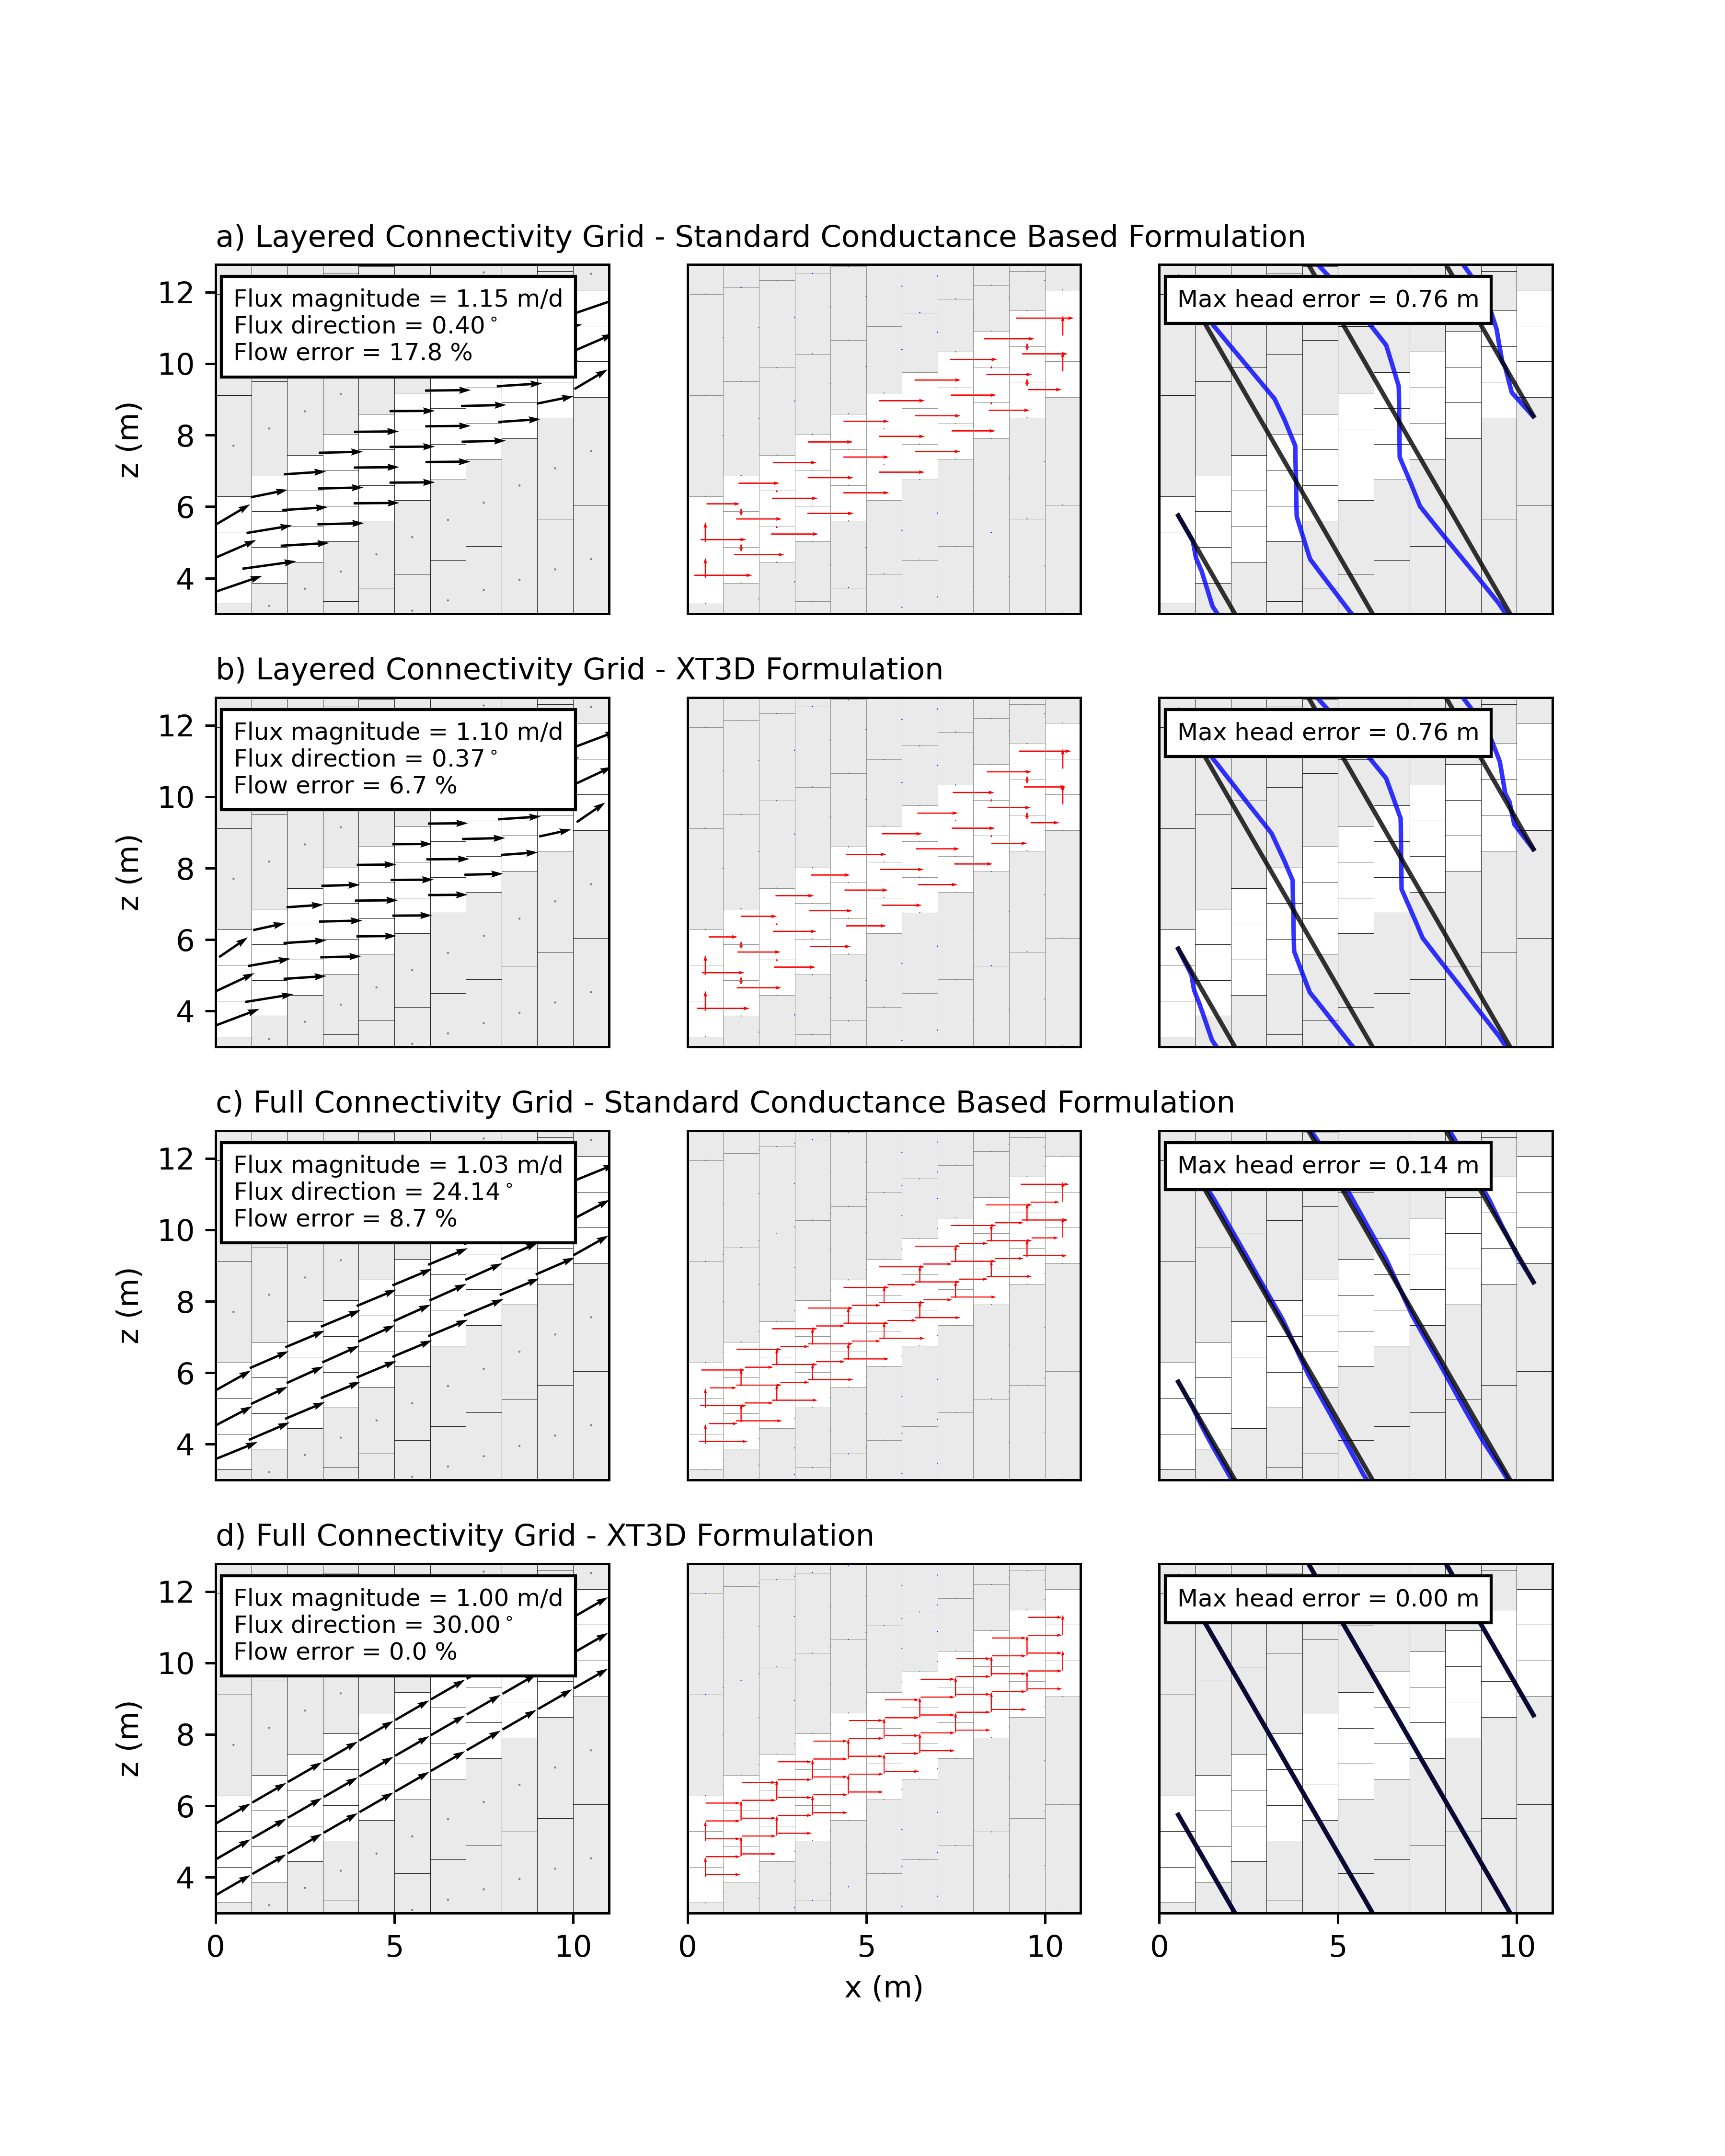
\includegraphics[scale=0.8]{../figures/fig2_paper.png}
	\caption{Numerical results for the test problem using base-case settings for layered-connectivity and full-connectivity grids, with the standard conductance based formulation as well as the XT3D formulation. The left panel of each scenario shows the calculated specific discharge at each cell centre (black arrows) with head contours (orange). The right panel shows the face flows (red arrows). {\color{red} (AMP: Change ``Vertically Offset'' to ``Layered Connectivity'' and ``Vertically Staggered'' to ``Full Connectivity'' in the script that generates the figure)} {\color{red} (AMP: Magnify tiny vectors in the domain [by the conductivity contrast, say] so they can be seen? Face flows along the aquifer/domain boundary are tricky because they're ``in between'' in terms of magnitude.)}}
	\label{fig:fig2}
	\end{center}
\end{figure}

\subsection{Effects of Grid Resolution}

{\color{red} Should we also consider the horizontal discretisation too? (CDL: I would say no.  Paper is already getting a bit long.) (AMP: I agree with CDL.  But let's be sure to mention that we've only looked at square cells in the aquifer.)}

\begin{figure}
	\begin{center}
	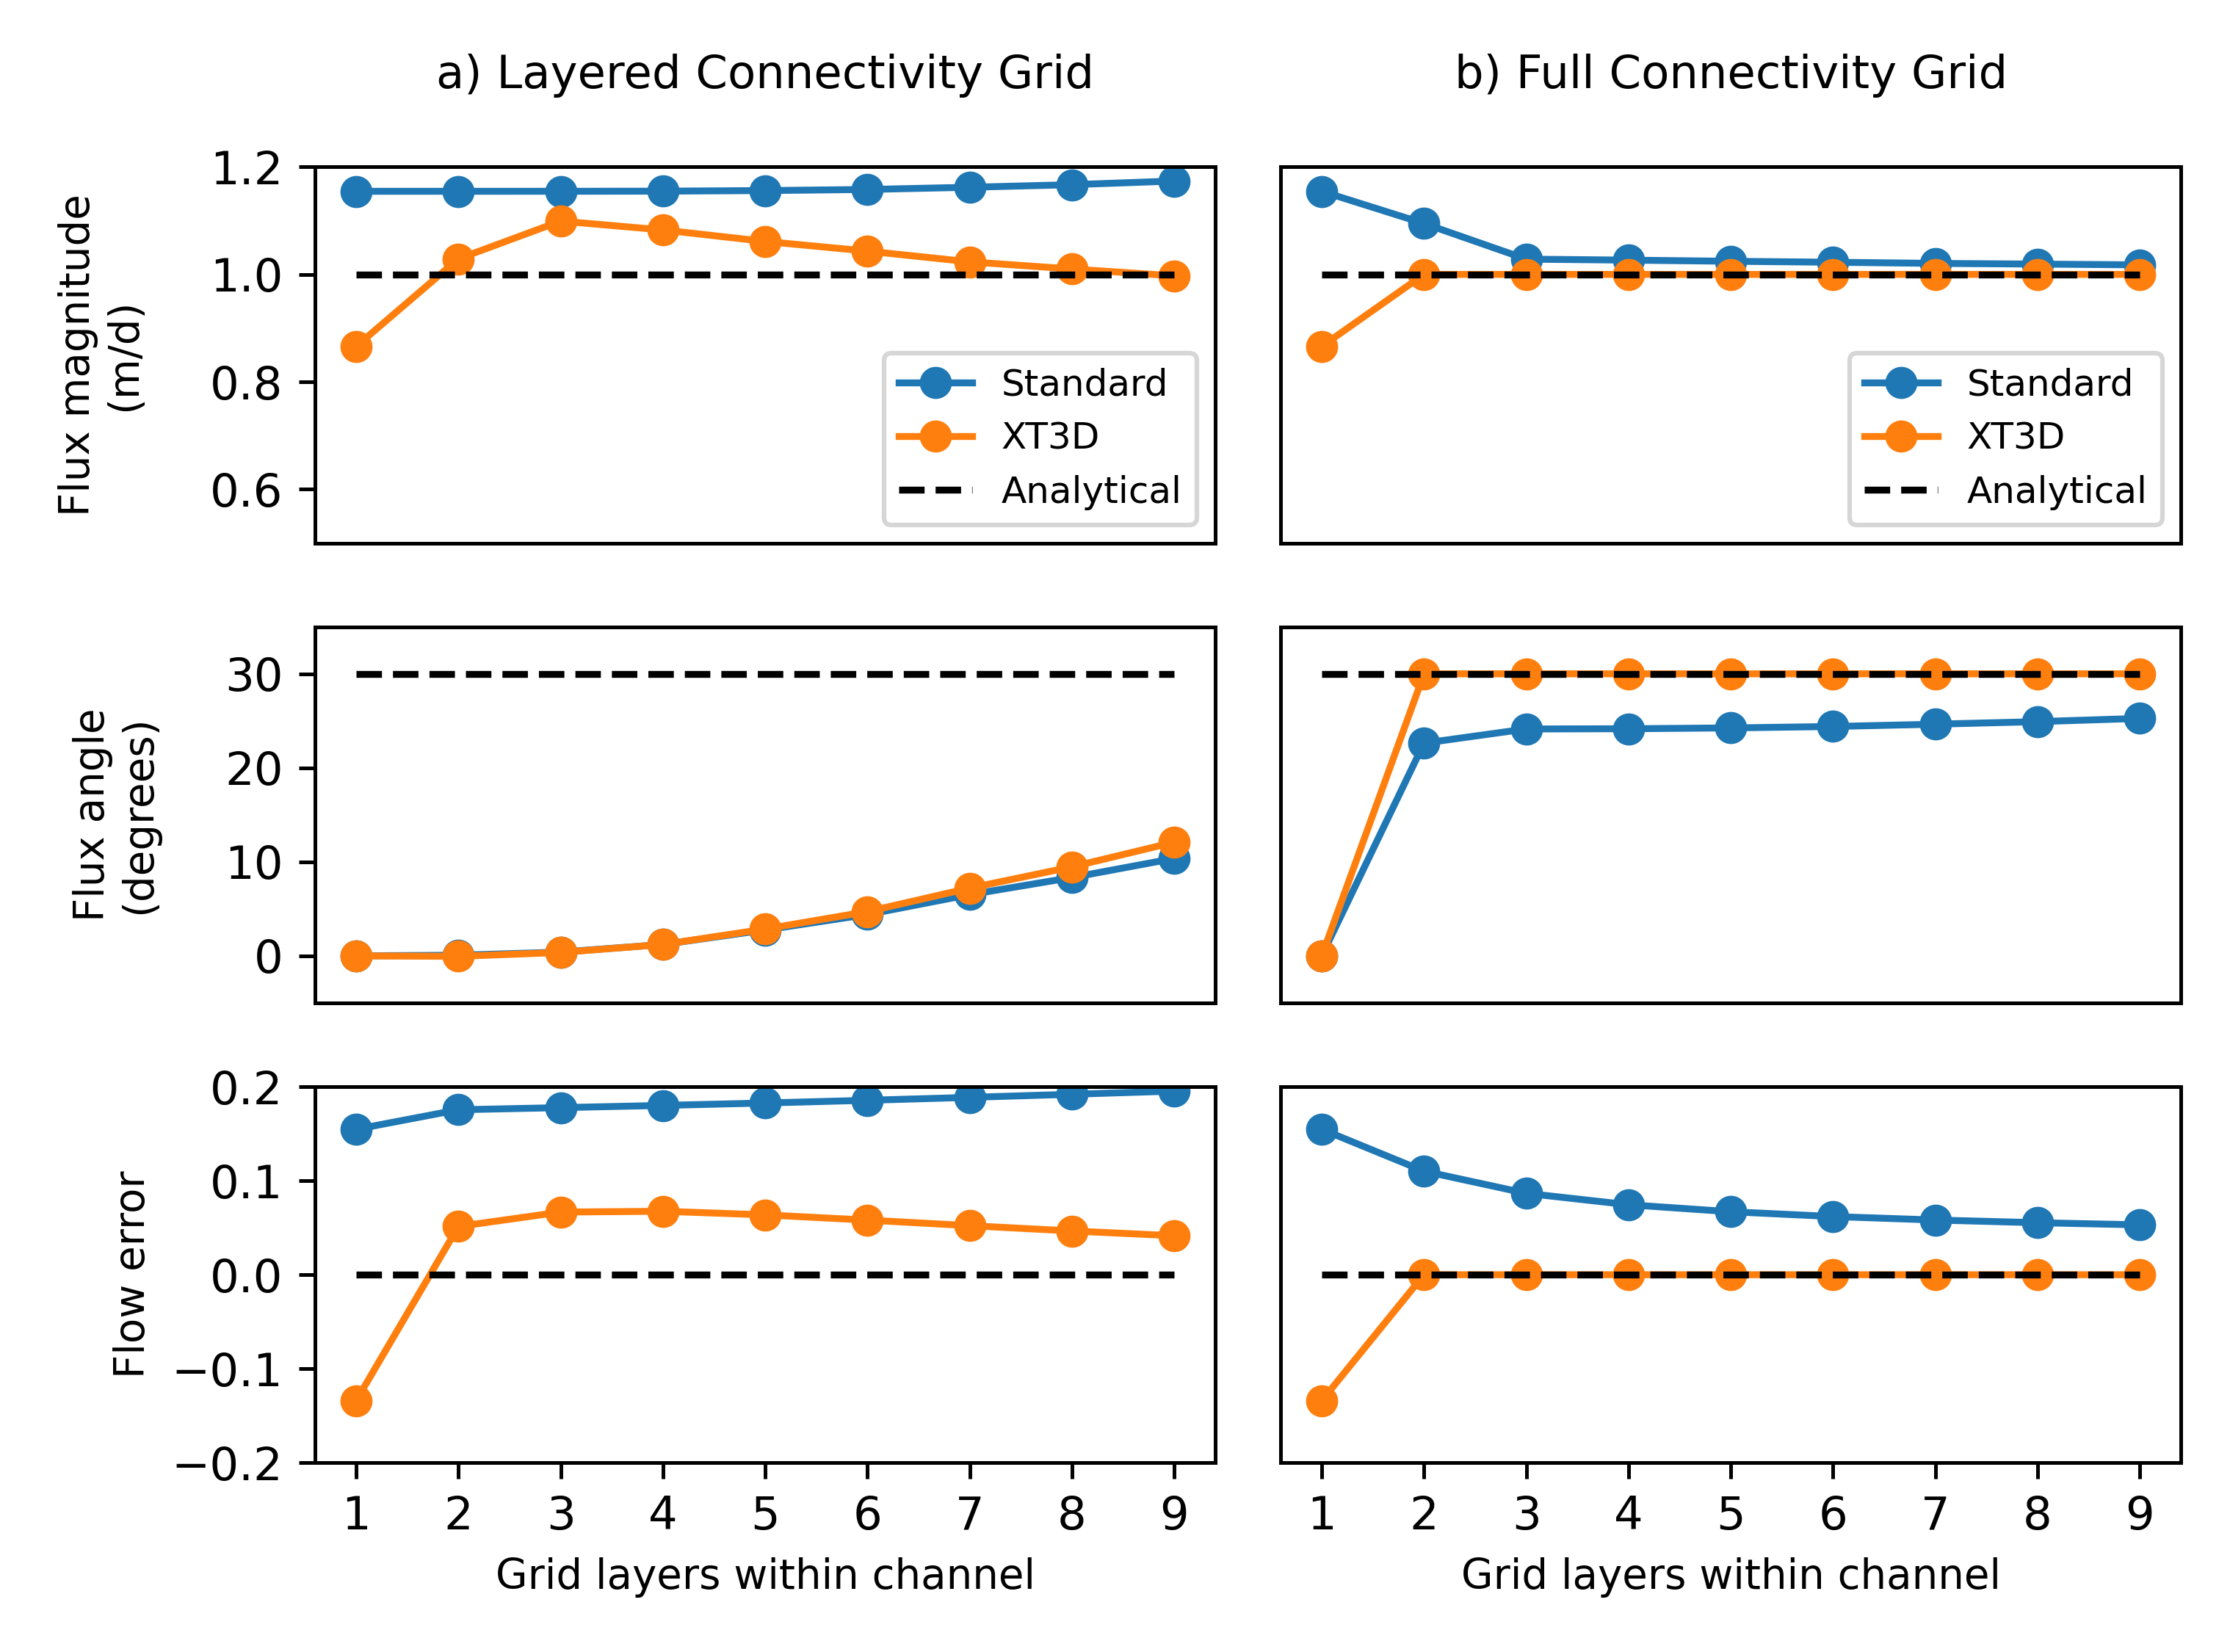
\includegraphics[scale=0.9]{../figures/fig3paper.png}
	\caption{Graphs indicating how increasing the number of grid layers within a single hydrogeologic layer (in this case, the aquifer) affects (a) flux magnitude of middle cell, (b) flux direction of middle cell and (c) volumetric flow through the hydrogeologic layer. We immediately notice the errors layered-connectivity grids incur (blue line), and how using a full-connectivity grid reproduces the analytical solution from two grid layers used to discretise the hydrogeologic layer (orange). {\color{red} (AMP: Change ``Vertically Offset'' to ``Layered Connectivity'', ``Vertically Staggered'' to ``Full Connectivity'', and ``Model layers'' to ``Grid layers'' in the script that generates the figure)}}
	\label{fig:fig3}
	\end{center}
\end{figure}

The base case arbitrarily uses 3 grid layers to represent the aquifer, but it is important to address the question: \emph{How many grid layers are required to adequately represent a hydrogeological layer?}. Layered-connectivity grids, which have been used by groundwater modellers for decades (ref?) {\color{red} Jim to check, I think there is some refinement guidance for aquitards}, are almost always configured as one grid layer per hydrogeological unit. {\color{red} (AMP: Could maybe mention that it's generally well known you want multiple layers for accurate transport?)} However, although computationally efficient, we investigate the effect of altering resolution within the aquifer by using the base case and varying number of cells per aquifer width from one to nine {\color{red} (AMP: Explain how aquifer and domain dimensions vary with the discretization. And is that how we want them to vary?)} Figure \ref{fig:fig3}). {\color{red} (AMP: Are all results in this figure with XT3D? If so, would there be any benefit to showing the standard formulation results, as well?)} We compare modeled flux magnitude and direction in the center cell, as well as the volumetric flow against the analytical solution. {\color{red} (AMP: Should we also say something about the error in the head solution? Report the maximum head error in each case?)}

Flux magnitude error for layered-connectivity grids peaked at around 10\% but improved and tended to zero with refinement. Flux direction for layered-connectivity grids is clearly a major issue, being reported as horizontal for one grid layer per aquifer width, and only improved to 12$^{\circ}$ for 9 grid layers per aquifer width. Flow through the aquifer peaked at 13\% error but decreased to only a 4\% error for 9 grid layers per aquifer width.

The results for the full-connectivity grid clearly show that a minimum of two grid layers per aquifer width is required to match the analytical result for flux magnitude, direction and volumetric flow. This is an important finding as it demonstrates that computational efficiency can be made using a full-connectivity grid over a rectilinear grid overlay approach, but it is important to use a minimum of two grid layers per hydrogeological unit to allow vertical fluxes to be incorporated into the flow solution. 

\subsection{Effects of Dip Angle and Conductivity Contrast}

The base case uses a dip angle of 30$^{\circ}$ and an extreme conductivity contrast between aquifer and domain of 1:$10^{-6}$. Here, we investigate the behavior of the flow solution for a wide range of aquifer inclines by systematically changing the dip angle by 2.5$^{\circ}$ from 0 to 80$^{\circ}$. Similarly, we examine the solution for multiple conductivity contrasts by changing the domain conductivity to 2, 5, 10 and 100 times less than the aquifer. {\color{red} (AMP: Dare we try making the domain more conductive than the ``aquifer''?)}  Simulated flux magnitude and direction of the centre cell for all combinations are plotted against the analytical solution in Figure \ref{fig:fig4}. 

Traditional layered-connectivity grids without XT3D shows rapid diversion of flux magnitude and direction from the analytical solution as dip increases (Figure \ref{fig:fig4a}). Use of the XT3D option keeps the flux magnitude somewhat on-track until about 30$^{\circ}$ when the solution starts peeling away from the analytical. Flux direction is improved for the homogeneous scenario, but not for the heterogeneous scenarios. The full-connectivity grid on the other hand, even without XT3D, roughly follows the analytical solution for flux magnitude and direction until around 65$^{\circ}$ when it starts to ``fall-apart.'' There are also spikes at certain dip angles which are related to transitions between cell connections due to changing cell face overlaps. The full-connectivity grid with XT3D clearly boasts the best results with the flux magnitude and direction matching the analytical until 65$^{\circ}$, with the exception of a slight decrease in flux direction after 45$^{\circ}$. {\color{red} (AMP: Can explain the wheels coming off around 65 deg by the fact that with only 3 cells vertically in the aquifer, the aquifer then looks like a long, zigzag Tetris piece that's no more than one cell wide, either vertically or horizontally.  Finer vertical discretization improves things.)}

These results confirm that full-connectivity grids with XT3D not only outperform the alternatives when modelling dipping hydrogeological unit, but come extremely close to the analytical solution.

\begin{figure}[p!]
\centering
\begin{subfigure}{0.9\textwidth}
	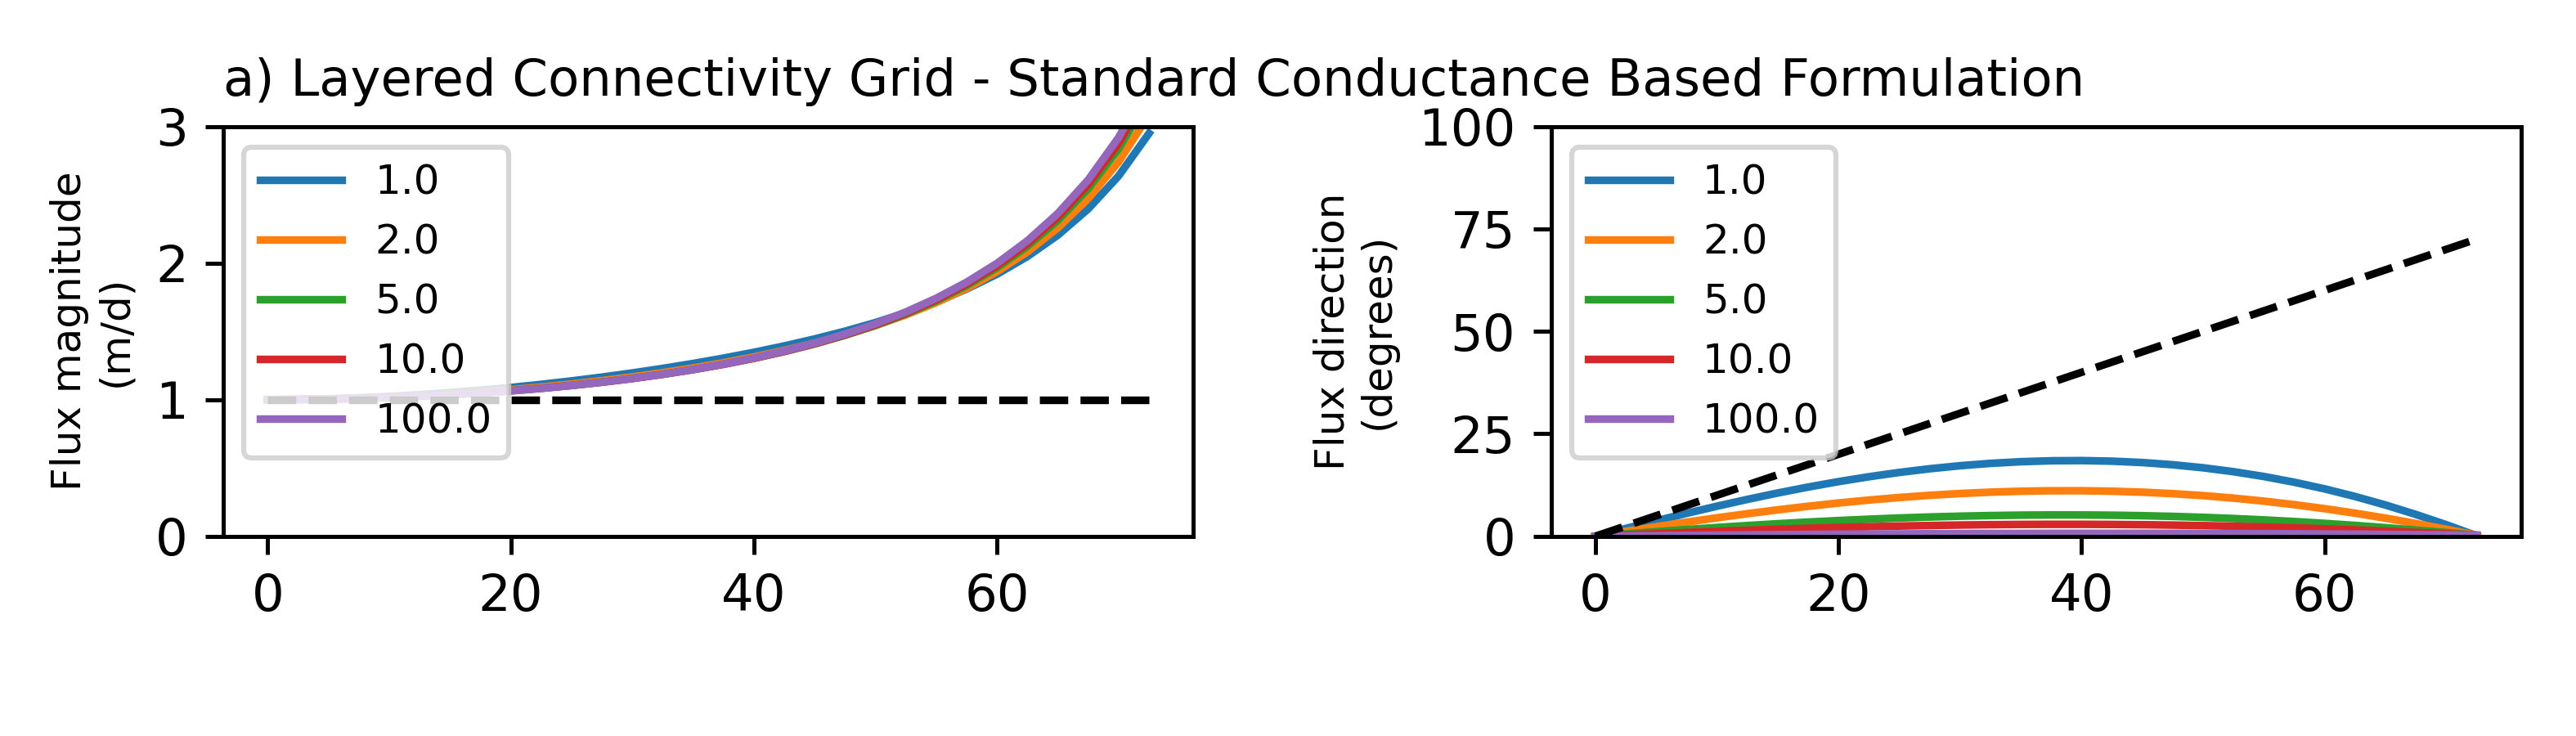
\includegraphics[width=\textwidth]{../figures/fig4_0_paper.png}
	\caption{layered-connectivity grid, standard conductance-based formulation}
	\label{fig:fig4a}
\end{subfigure}
\begin{subfigure}{0.9\textwidth}
	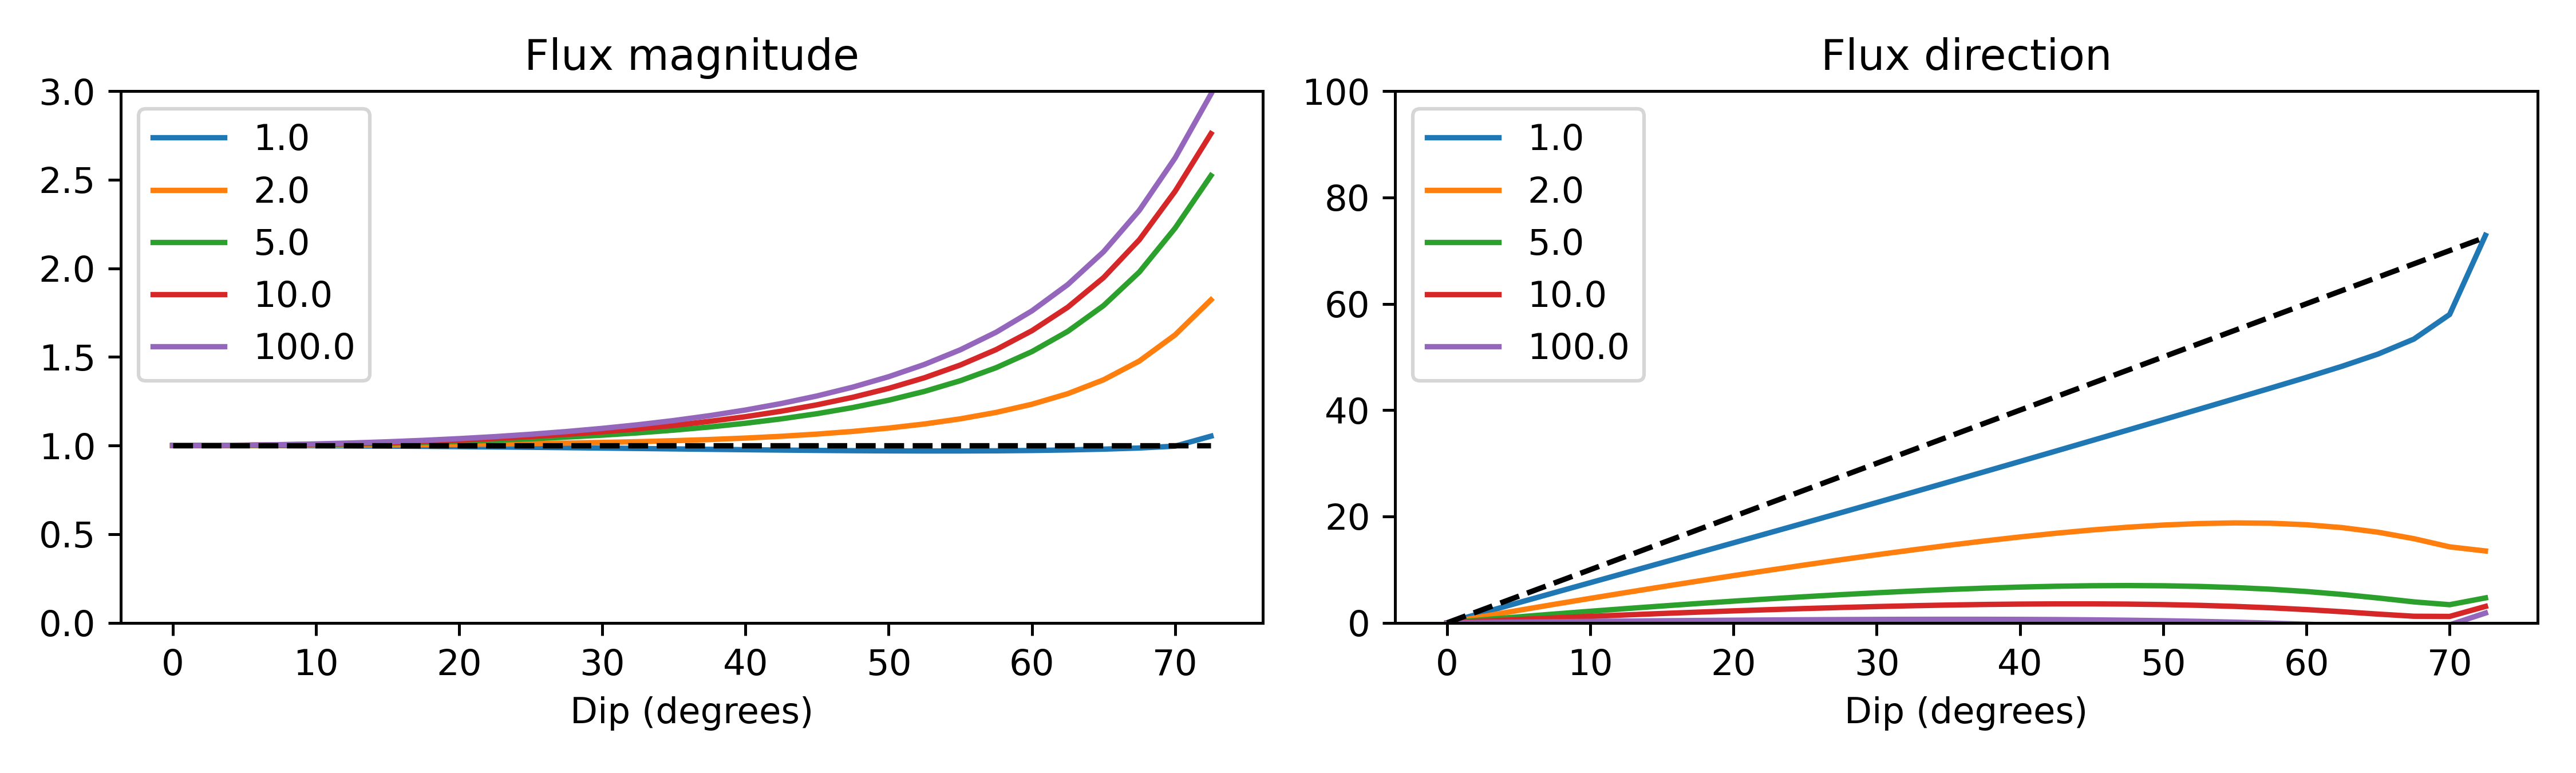
\includegraphics[width=\textwidth]{../figures/fig4_1_paper.png}
	\caption{layered-connectivity grid, XT3D}
	\label{fig:fig4b}
\end{subfigure}
\begin{subfigure}{0.9\textwidth}
	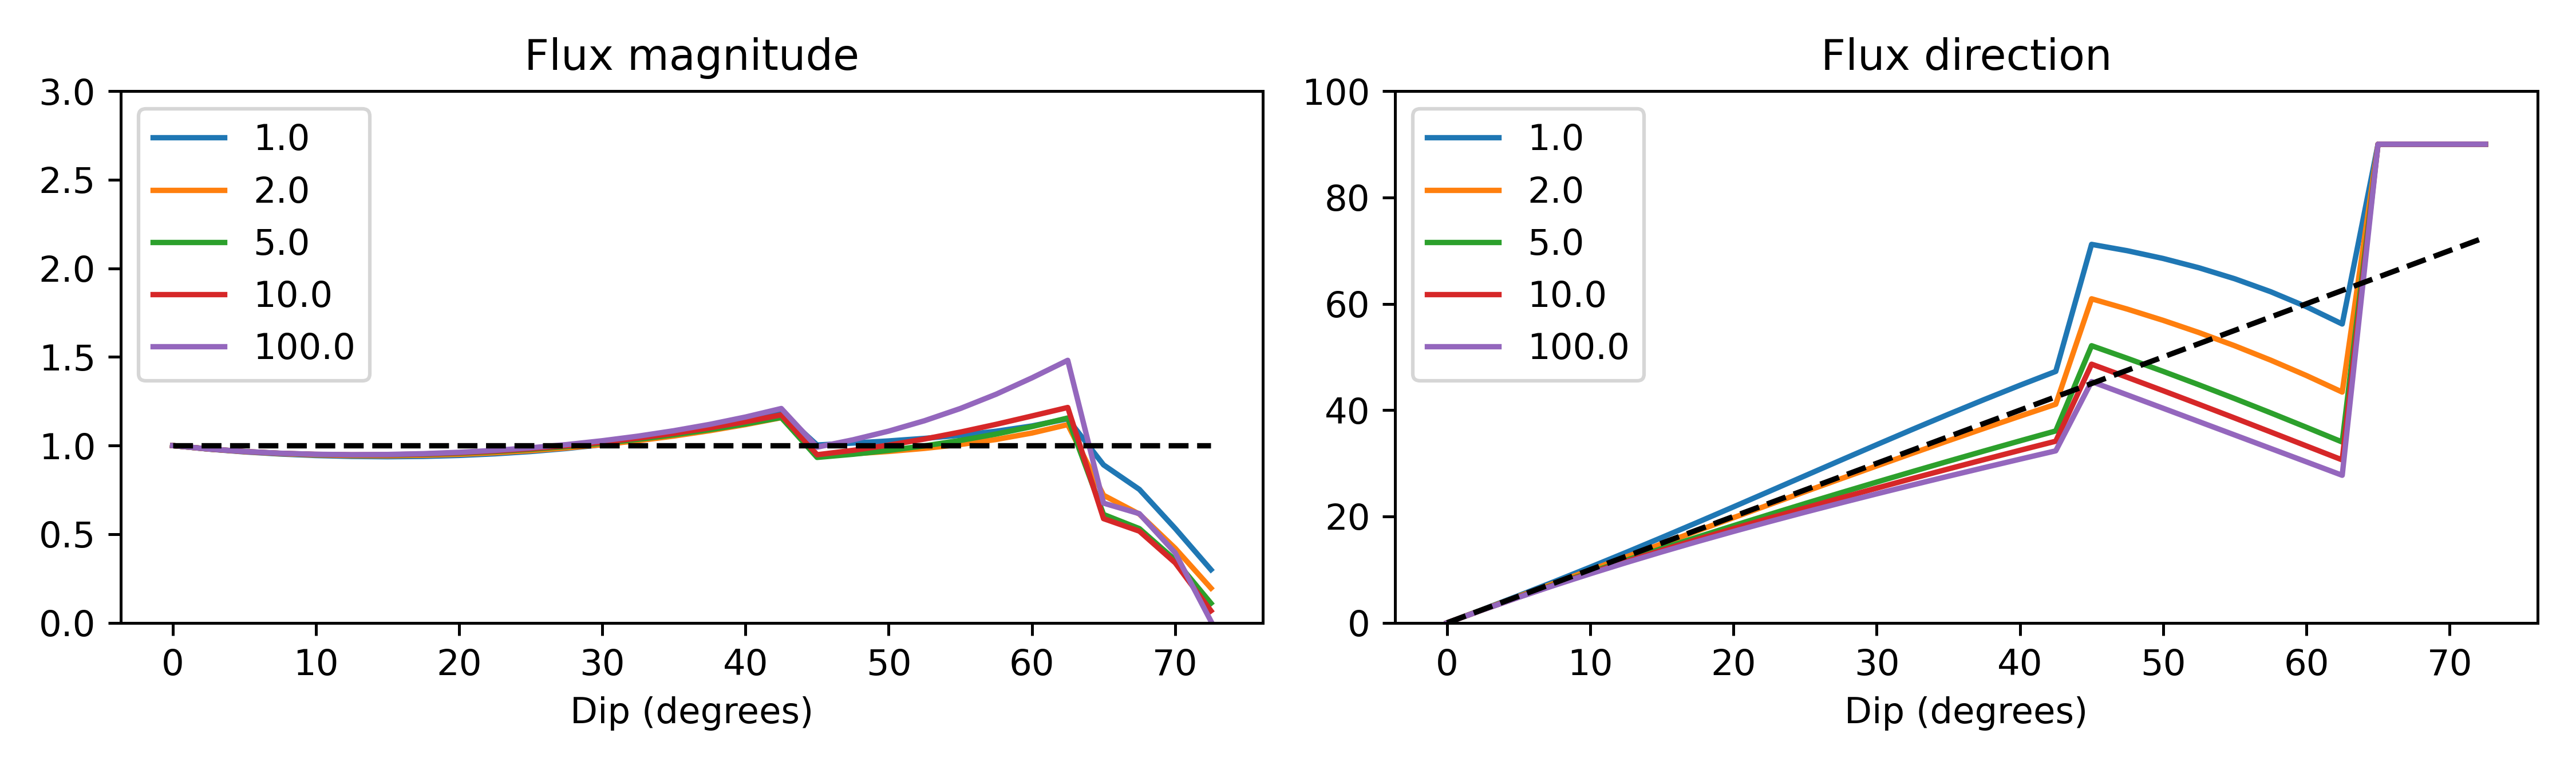
\includegraphics[width=\textwidth]{../figures/fig4_2_paper.png}
	\caption{full-connectivity grid, standard conductance-based formulation}
	\label{fig:fig4c}
\end{subfigure}
\begin{subfigure}{0.9\textwidth}
	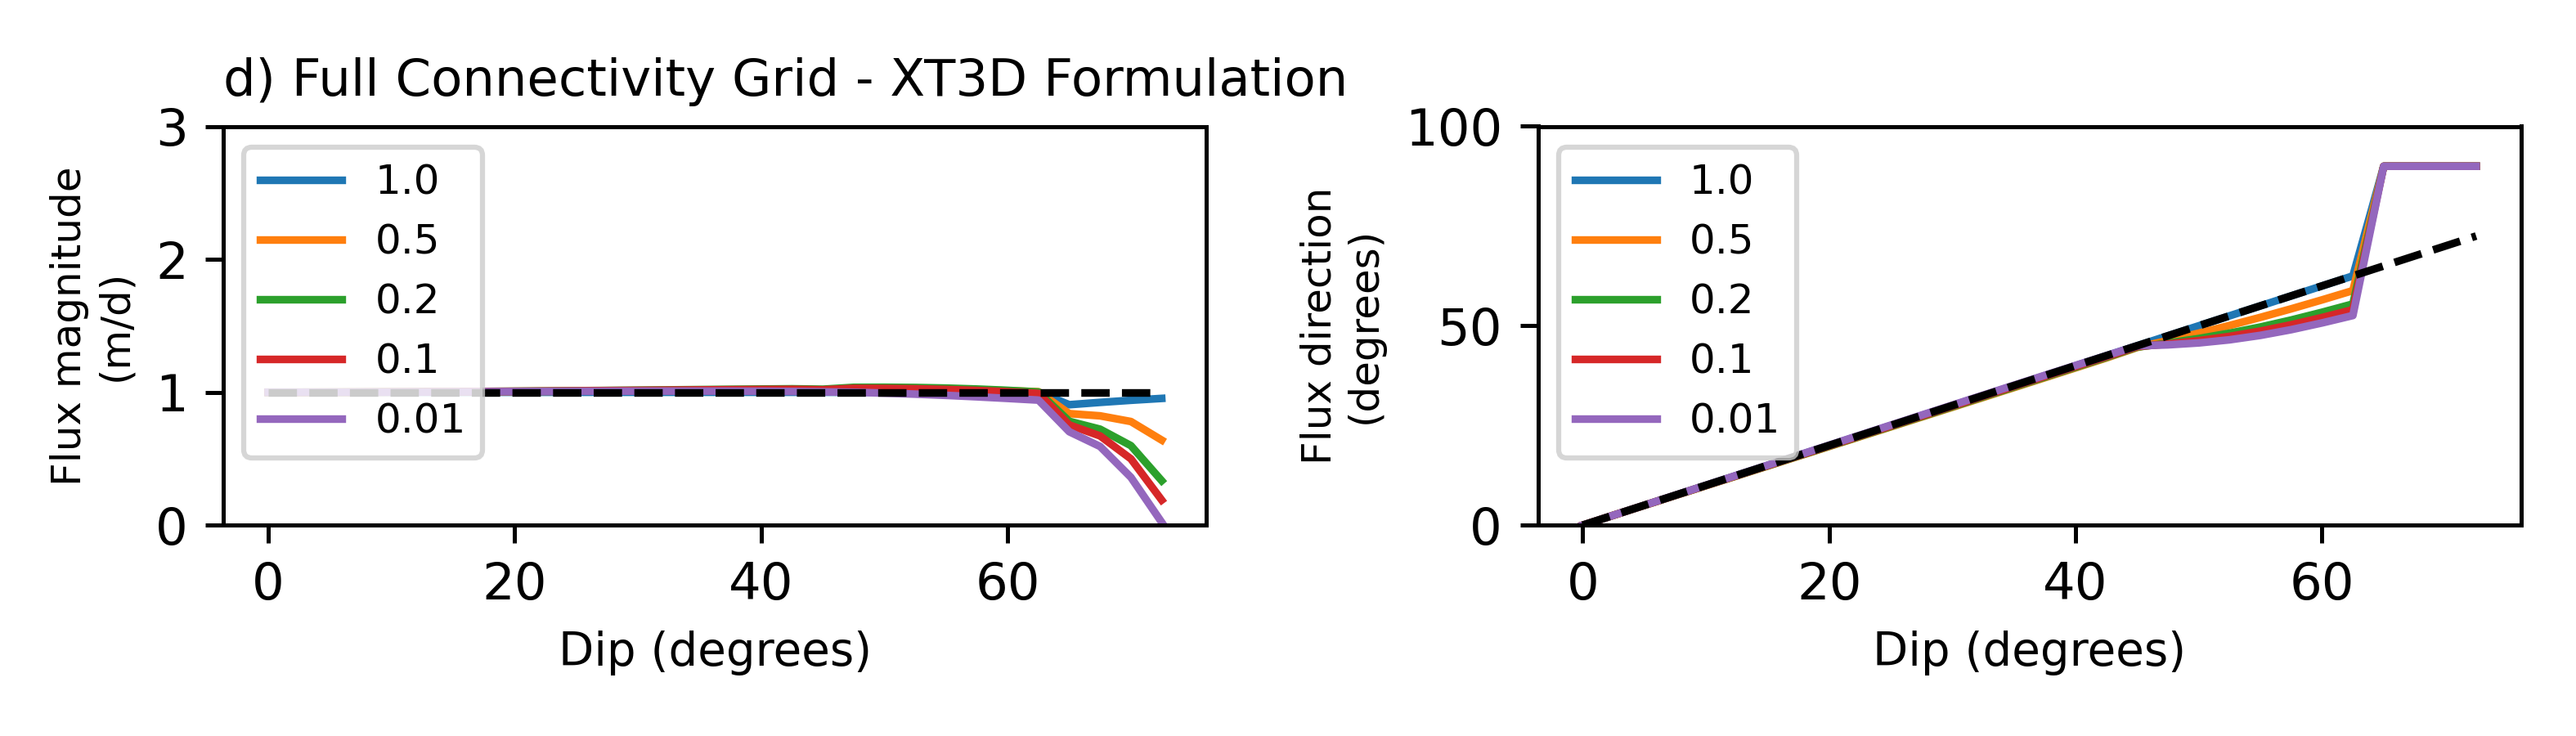
\includegraphics[width=\textwidth]{../figures/fig4_3_paper.png}
	\caption{full-connectivity grid, XT3D}
	\label{fig:fig4d}
\end{subfigure}

\caption{Flux magnitude and direction for centre cells for varying contrasts in log conductivity (blue, orange, green, red lines) for varying dip angles (x-axis). The analytical value is shown in black dashed line.}
\label{fig:figures}
\end{figure}

\subsection{Effect of Anisotropy}

The base case and subsequent scenarios have assumed isotropic conductivity. However, sedimentary layers often exhibit anisotropic conductivity, and therefore we examine the gridding strategies using anisotropic and dipping conductivity tensors {\color{red} (AMP: in the domain and aquifer, or only in the aquifer?)}, with reduced conductivity perpendicular to the aquifer by 10, 100, 1000 and 10,000. We also include the isotropic scenario (ratio of 1). {\color{red} (AMP: Dare we try increased perpendicular conductivity?)} Results are presented in Figure \ref{fig:fig5}. {\color{red} (AMP: Are all results in this figure with XT3D? If so, would there be any benefit to showing the standard formulation results, as well?)} Layered-connectivity grids produce flux magnitude and flow results that significantly deviate from the analytical solution (blue line), whilst full-connectivity grids reproduce the analytical solution (orange line). These results verify, once again, our proposed method of using full-connectivity grids to model dipping anisotropic hydrogeologic layers.


\begin{figure}
	\begin{center}
	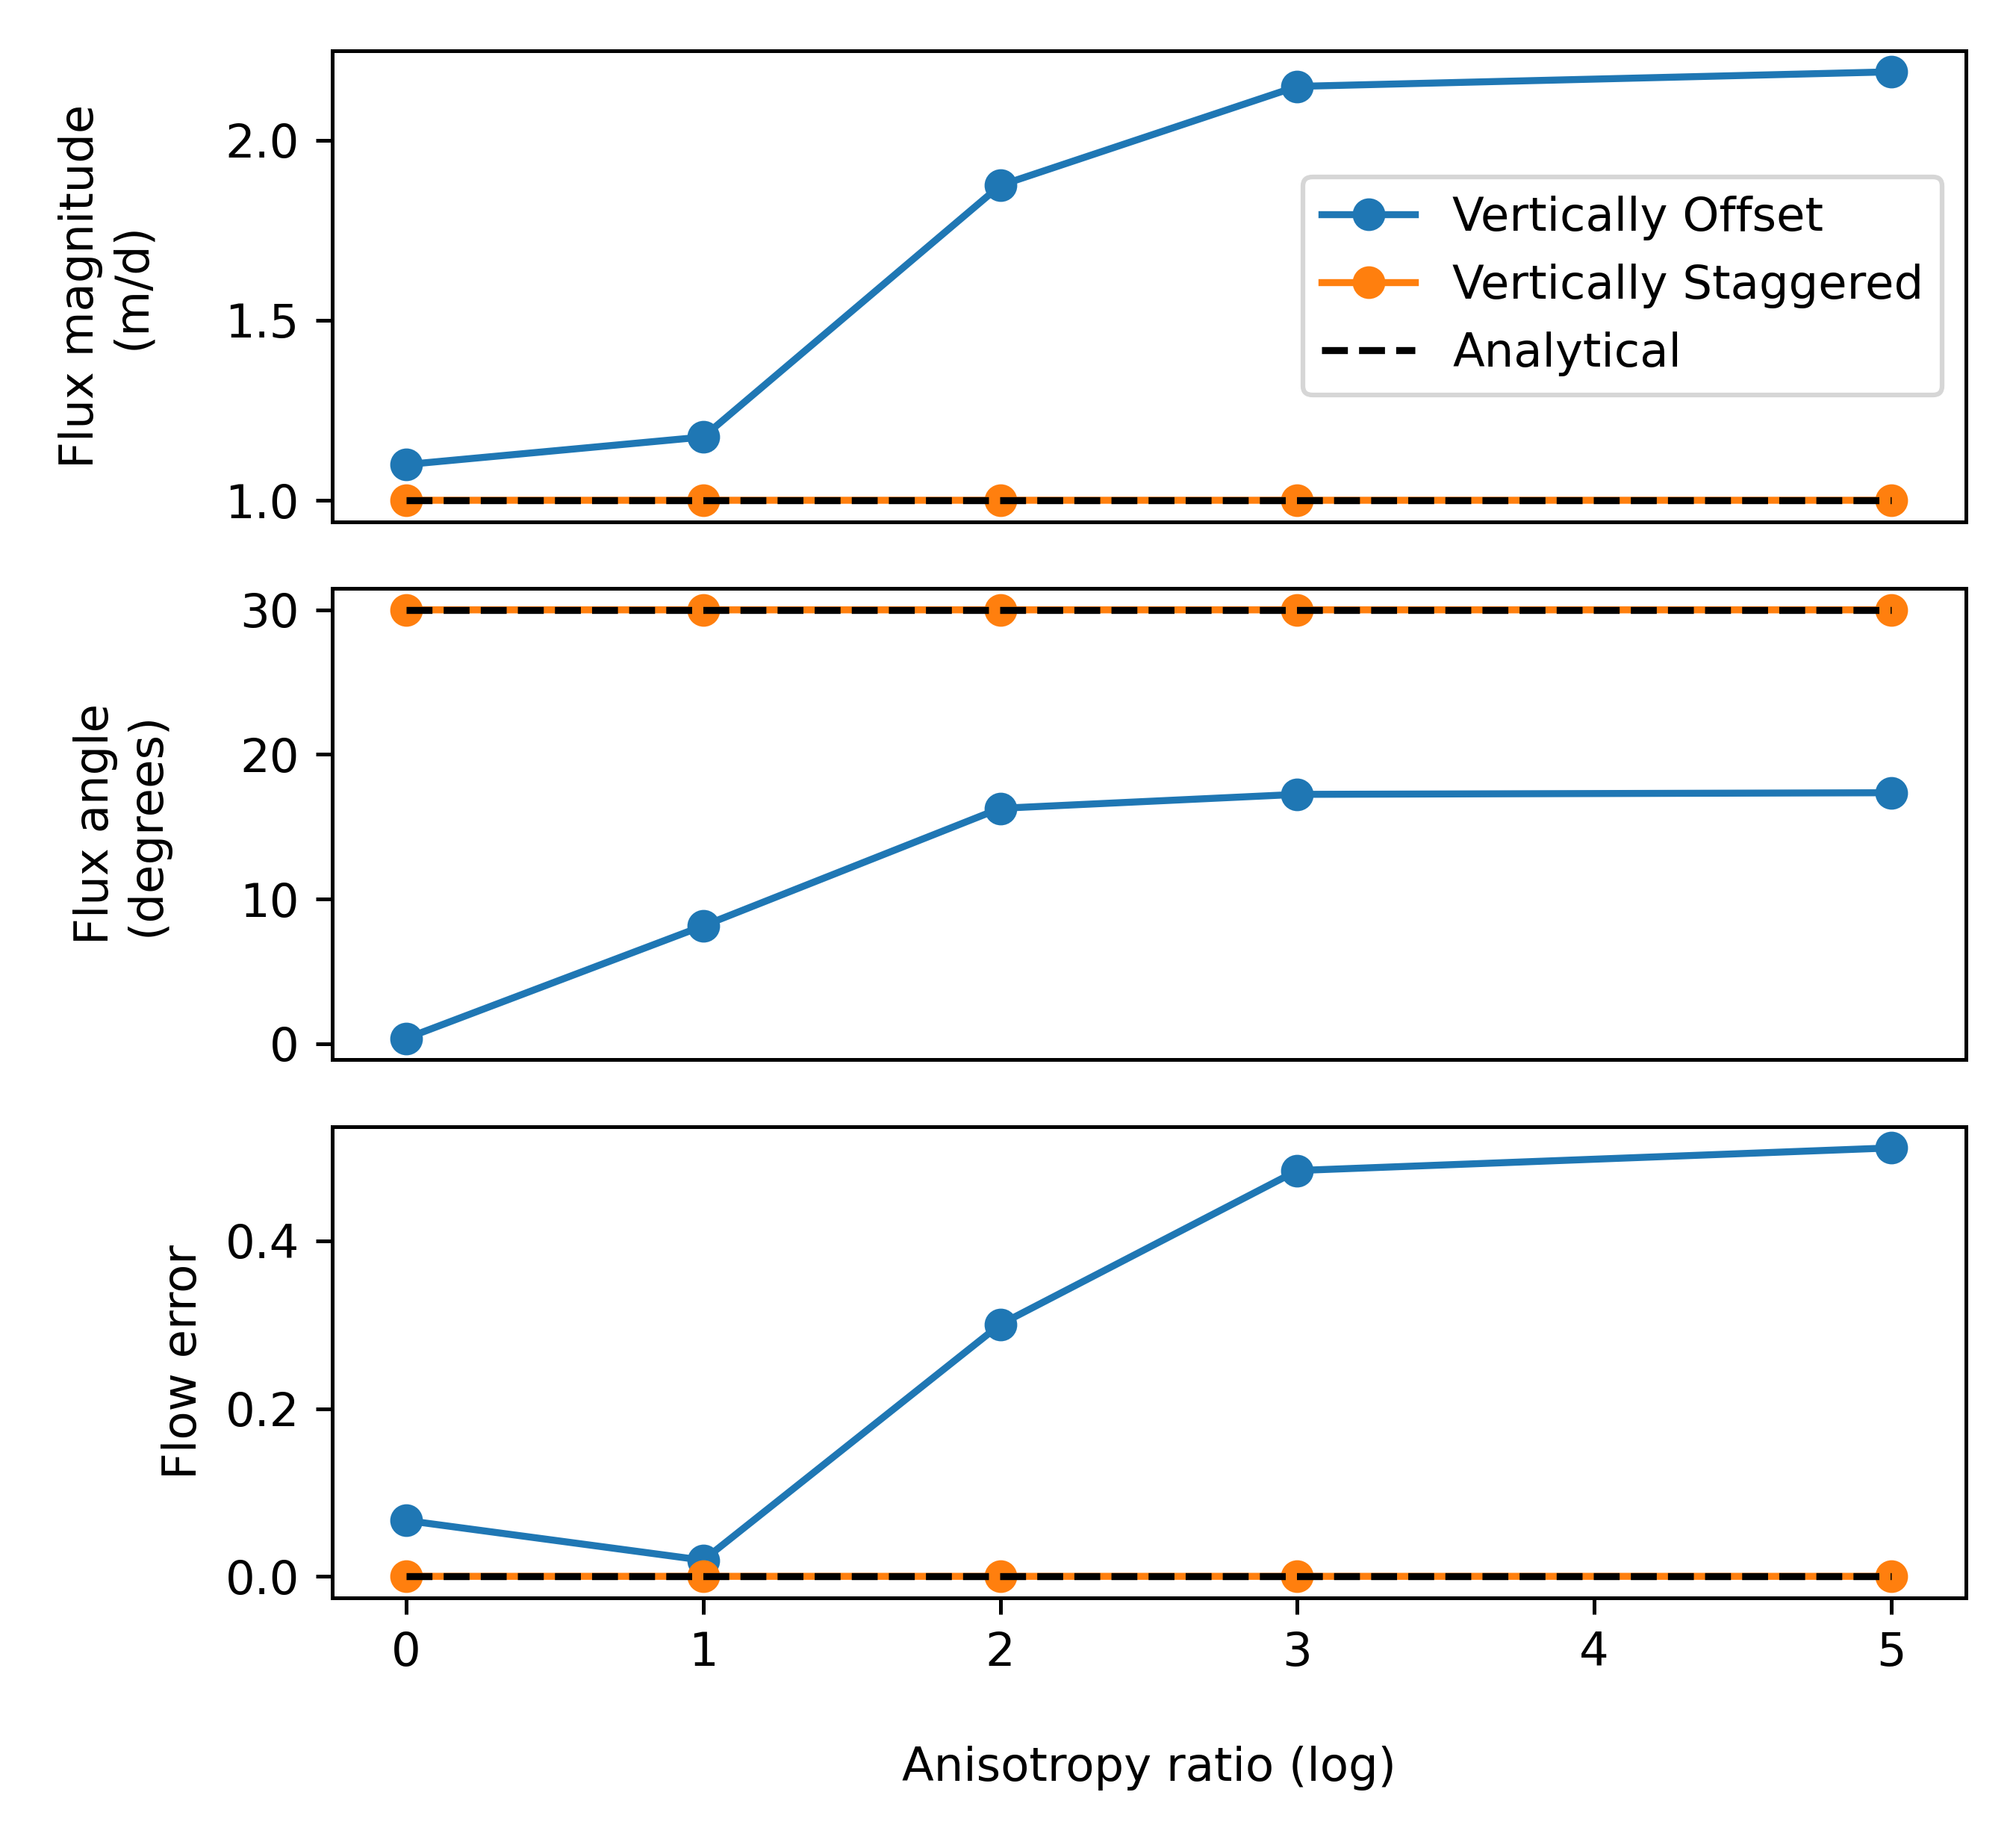
\includegraphics[scale=0.9]{../figures/fig5paper.png}
	\caption{Varying anisotropy ratios of conductivity withing the aquifer and the resulting (a) flux magnitude of middle cell, (b) flux direction of middle cell and (c) volumetric flow through the aquifer. }
	\label{fig:fig5}
	\end{center}
\end{figure}


\section{Conclusions}

 {\color{red} CDL: I added the following two paragraphs in an attempt to summarize my understanding of the main conclusion.  Feel free to edit or scrap as you see fit.}

\cite{bardot2022} revisited the capability of MODFLOW to accurately simulate groundwater flow through sedimentary structures.  They concluded that the XT3D multi-point flux approximation in MODFLOW 6 significantly improves the accuracy of simulated flows when used with a grid-overlay approach in which locations of sedimentary structures, which can be steeply dipping, are mapped onto a relatively fine, rectilinear model grid.  They also concluded that the XT3D multi-point flux approximation does not perform as well as anticipated when simulating flow through a steeply dipping hydrogeologic layer using vertically offset grids, which are advantageous for significantly reducing the number of grid layers required for many problems.  They hypothesized that the inherently limited lateral connectivity between cells in DIS and DISV layered grids in MODFLOW 6 was responsible for the inability to obtain accurate flow results in their steeply dipping test problems using vertically offsets grids, with or without XT3D.

In this paper, we have confirmed that the layered lateral connectivity implemented in DIS and DISV model grids is inadequate for simulating groundwater flow through steeply dipping sedimentary structures, even when the XT3D multi-point flux approximation is used.  However, when connections between laterally adjacent cells in different grid layers are added to comprise a grid with full connectivity, there is a substantial increase in the accuracy of simulated flows.  The additional connectivity is implemented using the fully unstructured (DISU) grid type.  Importantly, this accuracy improvement requires that at least two grid layers be used to represent the steeply dipping sedimentary structure.  The primary conclusion of this paper is that, given appropriate discretization and cell connectivity, the XT3D multi-point flux approximation implemented in MODFLOW 6 can be combined with vertically offset grids to efficiently and accurately model flows through {\color{red} steeply dipping??} sedimentary structures.  Prior to this work, the capability to efficiently and accurately model flow through {\color{red} steeply dipping??} sedimentary structures was generally restricted to finite element simulators.

The importance of adequate connectivity has been explained and evaluated in this work specifically in terms of hydrogeologic layers that correspond to sedimentary structures. However, the impact of cell connectivity on the accuracy of simulated flows should be considered in any MODFLOW application that models flow through a heterogeneous hydraulic conductivity field using a grid with large vertical offsets between laterally adjacent cells, whether or not the grid has a layered structure. The full connectivity needed to improve accuracy can be implemented using the DISU grid types in both MODFLOW 6 and MODFLOW-USG.

Points:

1) Furthermore, we point out the nuances in specific discharge calculations and the ambiguity introduced when assessing model behaviour.  MODPATH and MT3D

3) (Random thought) The use of full-connectivity grids improved the accuracy of the transect solutions; however, the results of \citep{bardot2022} using unstructured meshes that conformed to the aquifer geometry preformed better in isotropic grids. If you force the normal flux to be the same at the interface of the domain and aquifer, the analytical solution would suggest a uniform gradient either side, do we introduce an error if the faces don't align with the aquifer correctly?  Would figure \ref{fig:fig2} show a correction for this if the anisotropic scenario was tested?  {\color{red} (AMP: Is the underlying question whether using an unstructured mesh that conforms to the aquifer geometry [which MF6 can't do in transect] would improve the accuracy more than a full-connectivity vertically offset grid, assuming xt3d is used in both cases? Let's discuss on our next call.)}

 {\color{red} CDL: Maybe worthwhile to implement full connectivity approaches for DIS and DISV grids in mf6.}

\section{Acknowledgments}
We would like to acknowledge.... {\color{red} that this simple paper has been in the works far too long. Kindly address complaints to the first author.}

\section{Supporting Information}

\section{Appendix}

\bibliography{references.bib}


\end{document}
